% TODO: Fix dirty hack in thwregex.sty, where I changed line 42 to print star in math-mode
% 		because otherwise the star was always raised in my config.
%		Use \rx everywhere

% This slide is only here because \only dosn't work in Title
\ifdefined \handout \else
\begin{frame}{}
	Gibt es einen endlichen Akzeptor mit $$L = \{ a^kb^k | k\in \nN_0 \}$$ 
	% This is to reserve the space so the text doesn't jump
	\visible<0>{Nein! Warum nicht?\\
		
		Gibt es einen endlichen Akzeptor, der alle gültigen Klammerausdrücke erkennt?\\
		Nein, aus dem selben Grund.
		\begin{figure}[H]
			
\includegraphics[scale=0.5]{xkcd/tags_1144}
			\caption{ \texttt{\url{https://www.xkcd.com/1144/}} }
		\end{figure}
		Kontextfreie Grammatiken \enquote{können also mehr} als endliche Automaten.\\
		Wir wollen nun ein \enquote{gleichmächtiges} Konzept.}
\end{frame}
\fi

\begin{frame}{Grenzen endlicher Automaten}
	Gibt es einen endlichen Akzeptor mit $$L = \{ a^kb^k | k\in \nN_0 \}$$ 
	Nein! Warum nicht?\\
	
	Gibt es einen endlichen Akzeptor, der alle gültigen Klammerausdrücke erkennt?\\ \pause
	Nein, aus dem selben Grund.
	\begin{figure}[H]
		
\includegraphics[scale=0.5]{xkcd/tags_1144}
		\caption{ \texttt{\url{https://www.xkcd.com/1144/}} }
	\end{figure}
	\pause
	Kontextfreie Grammatiken \enquote{können also mehr} als endliche Automaten.\\
	Wir wollen nun ein \enquote{gleichmächtiges} Konzept.
\end{frame}

\section{Reguläre Ausdrücke}
\subsection{Definition}

\begin{frame}{Reguläre Ausdrücke}
	Wir können uns reguläre Ausdrücke zusammenbauen aus
	\begin{itemize}[<+->]
		\item den einzelnen Symbolen $x$ aus $A$
		\item zwei regulären Ausdrücken $R_1$ und $R_2$ mit $$(R_1 R_2) \qquad \text{ oder } \qquad (R_1 \mid R_2)$$
		\item einem Stern $R\ast$
		\item oder dem leeren Ausdruck
	\end{itemize} \pause
	Klammern dürfen nach den Klammerregeln weggelassen werden:\\
	Stern vor Punkt vor Strich.
\end{frame}

\begin{frame}{Reguläre Ausdrücke}
	\begin{Beispiel}
		Sei $ A = \{ a, b, c\}$. Dann sind gültige reguläre Ausdrücke:\\
		$\rx{abc}$\\
		$\rx{a|b|c}$\\
		$\rx{(ab)*}$\\
		$\rx{O*}$
	\end{Beispiel}
\end{frame}


\begin{frame}{Sprache eines Ausdruckes}
	Die durch $R$ beschriebene Sprache $\lang{R}$ ist wie folgt definiert:
	\begin{itemize}
		\item $\lang{\rx{O}} = \emptyset$
		\item $\lang{x}=\{x\} \; (x\in A)$
		\item $\lang{R_1 \rx| R_2} = \lang{R_1} \cup \lang{R_2}$
		\item $\lang{R_1 R_2} = \lang{R_1} \cdot \lang{R_2}$
		\item $\lang{R\rx*} = \lang{R}^*$
	\end{itemize} 
\end{frame}

\begin{frame}
	\begin{Beispiel}
		\begin{itemize}[<+->]
			\item $\lang{\rx{a}} = \{\#a\}$
			\item $\lang{\rx{ab}} = \lang{\rx{a}} \cdot \lang{\rx{b}} = \{\#a\#b\}$
			\item $\lang{\rx{a|b}} = \lang{\rx{a}}\cup\lang{\rx{b}} = \{\#a,\#b\}$.
			\item $\lang{\rx{(a|b)*}} = \lang{\rx{a|b}}^* = \{\#a,\#b\}^*$.
			\item $\lang{\rx{(a*b*)*}} = \lang{\rx{a*b*}}^* = (\lang{\rx{a*}}\lang{\rx{b*}})^* 
			= (\lang{\#a}^*\lang{\#b}^*)^* = (\{\#a\}^*\{\#b\}^*)^*$\\
			$= \{\#a,\#b\}^*$. 
		\end{itemize}
	\end{Beispiel}
\end{frame}

\begin{frame}{Aufgabe: Reguläre Ausdrücke}
	In dieser Aufgabe geht um die formalen Sprachen
	$$L_1 = \{a^k b^m \mid k, m \in \nN_0 \} \qquad L_2 = \{b^k a^m \mid k, m \in \nN_0 \}$$
	Geben Sie für jede der folgenden formalen Sprachen $L$ je einen regulären Ausdruck $R$ an mit $ \langle R \rangle = L$.
	\begin{itemize}
		\item $L = L_1 \cup L_2$ 
			\only<2-|handout:2>{$\qquad a\ast b\ast \mid b\ast a\ast$}
		\item $L = L_1 \cap L_2$
			\only<3-|handout:2>{$\qquad a\ast \mid b\ast $}
		\item $L = L_1\cdot L_2$
			\only<4-|handout:2>{$\qquad a\ast b\ast b\ast a\ast$ oder $a\ast b\ast a\ast$}
		\item $L = L_1\ast$
			\only<5-|handout:2>{$\qquad (a\ast b\ast)\ast$ oder $(a\mid b)\ast$}
	\end{itemize}
\end{frame}

\begin{frame}{Aufgabe: Sprachen regulärer Ausdrücke}
	\begin{itemize}
		\item $\lang{\rx{(a|b)*abb(a|b)*}} =$
		\item $\lang{\rx{a**}} $
		\item $\lang{???} = \lang{R}^+$
		\item $\lang{???} = \{\eps\}$
		\item $\lang{???} = \{\ w \in \{a, b\}^* \mid |w|_b > 2 \} $
		\item $\lang{???} =$ Sprache aller Wörter über $a, b$, in denen das Teilwort ab nicht vorkommt.
	\end{itemize}
\end{frame}

\begin{frame}{Lösung}
	\begin{itemize}
		\item $\lang{\rx{(a|b)*abb(a|b)*}} = \{\#a, \#b\}^* \cdot \{\#a\#b\#b\} \cdot \{\#a, \#b\}^*$
		\item $\lang{\rx{a**}} = \{a\}^*$
		\item $\lang{R\rx{(}R\rx{)*}} = \lang{R}^+$
		\item $\lang{\rx{O*}} = \{\eps\}$
		\item $\lang{\rx{a*ba*ba*b(a|b)*}} = \{\ w \in \{a, b\}^* \mid |w|_b > 2 \} $
		\item $\lang{\rx{b*a*}} =$ Sprache aller Wörter über $a, b$, in denen das Teilwort ab nicht vorkommt.
	\end{itemize}
\end{frame}

\section{Rechtslineare Grammatiken}
\begin{frame}{Rechtslineare Grammatiken}
	\begin{Definition}
		Eine Grammatik $G = (N, T, S, P)$ nennt man \textbf{rechtslinear} wenn bei jeder Produktion auf der rechten Seite höchstens ein Nichtterminalsymbol und dieses nur als letztes Symbol steht.\\
		Alle Produktionen folgen dem Schema $$X \to w \quad \text{oder} \quad X \to wY$$ mit $w \in T^*, \; X,Y \in N$.
	\end{Definition}
\end{frame}

\begin{frame}{Reguläre Sprachen}
	\begin{Satz}
		Für jede formale Sprache $L$ sind die folgenden drei Aussagen äquivalent:
		\begin{itemize}
			\item $L$ kann von einem endlichen Akzeptor erkannt werden.
			\item $L$ kann durch einen regulären Ausdruck beschrieben werden.
			\item $L$ kann von einer rechtslinearen Grammatik erzeugt werden.
		\end{itemize}
	\end{Satz}
	
	Eine solche Sprache nennen wir \textbf{regulär}.
\end{frame}

\begin{frame}{Beispiele für Umwandlungen}
	Siehe Übung 13, WS 15/16
\end{frame}

\begin{frame}{Beispiele}
	$G = (\{X, Y, Z\}, \{a, b\}, X, P )$ mit $$P = \{X \to aX \mid bY \mid \varepsilon, Y \to aX \mid bZ \mid \varepsilon, Z \to aZ \mid bZ\}$$ ist eine rechtslineare Grammatik. Die Sprache ist \pause $$L(G) = \{ w \mid \forall v_1, v_2 \in \{a,b\}^\ast: w \neq v_1 bb v_2 \}$$ Der reguläre Ausdruck ist \pause $$R =  (a\mid ba)\ast (b \mid \emptyset *)  $$ der Automat ist 
\end{frame}

\begin{frame}
	\begin{figure}[H]
		\centering
		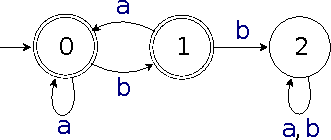
\includegraphics[width=\linewidth]{regulaer/L1.pdf}
	\end{figure}
\end{frame}

\begin{frame}
	Jetzt sieht man vielleicht auch $$G = (\{X\}, \{a, b\}, X, P )$$ mit $$P = \{X \to aX \mid baX \mid b \mid \varepsilon \}$$
\end{frame}

\begin{frame}{Noch mehr Beispiele}
	\begin{itemize}
		\item $G = (\{X \}, \{a, b\}, X , \{X \to abX \mid bbaX \mid \varepsilon \}$ wird beschrieben durch
			$L(G) = \lang{\visible<2-|handout:2>{ (ab\mid bba)\ast }} $
		\item $G = (\{X , Y\}, \{a, b\}, X , \{X \to aX \mid bX \mid ababbY , Y \to aY \mid bY \mid \varepsilon \}$ wird beschrieben durch 
			$L(G) = \lang{\visible<3-|handout:2>{ (a\mid b)\ast ababb(a\mid b)\ast }} $
	\end{itemize}
\end{frame}

\begin{frame}{Aufgabe}
	Gegeben ist im folgenden jeweils eine Beschreibung einer formalen Sprache $L$ und ein dazugehöriges Alphabet. Schreiben Sie jeweils den regulären Ausdruck $R$ auf, für den $L(R) = L $ gilt und stellen Sie eine rechtslineare Grammatik $G$ auf, für die $L(G) = L $ gilt:
	\begin{itemize}
		\item Die Menge aller Worte über dem Alphabet $A=\{a,b,c\}$, die genau ein c enthalten. \\
		\visible<2-|handout:2>{
			\emph{Lösung}: $(a|b)*c(a|b)*$
		}
		\item Die Menge aller Worte über dem Alphabet $A=\{a,b\}$, bei denen die Anzahl der $b$ durch 3 teilbar ist. \\
		\visible<3-|handout:2>{
			\emph{Lösung}: $a*(ba*ba*ba*)*$
		}
	\end{itemize}
\end{frame}

\begin{frame}{Aufgabe}
	\textit{Gegeben sei die rechtslineare Grammatik } $$ G= (\{S\},\{a,b\},S,P) \qquad P = \{S\to baaS | baS | aaS | \varepsilon \} $$
	\begin{itemize}
		\only<1-3|handout:1,2>{
			\item Geben Sie einen endlichen Akzeptor $A$ an, so dass $L(A) = L(G)$ gilt
			\only<3|handout:2>{
				\begin{figure}[H]
					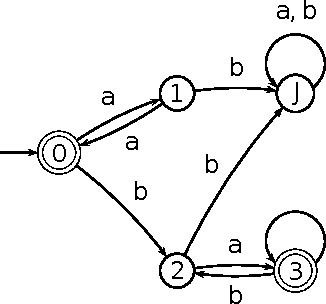
\includegraphics[scale=0.9]{regulaer/L2.pdf}
				\end{figure}
			}
		}
		\only<1,4-5|handout:1,3>{
			\item Geben Sie einen regulären Ausdruck $R$ an, so dass $ \langle R \rangle = L(G) $ gilt
			\only<5|handout:3>{
			$$ (baa|ba|aa)\ast$$
			}
		}
		\only<1,6-7|handout:1,3>{
			\item Geben Sie einen regulären Ausdruck $R$ an, der nicht das Zeichen $|$ enthält, und für den $\langle R \rangle = L(G) $ gilt.
			\only<7|handout:3>{
			$$ (aa)\ast (baa\ast)\ast $$
			}
		}
	\end{itemize}
\end{frame}



%\begin{frame}
%	\frametitle{Was wir können:}
%	Von..
%	\begin{description}
%		\item[..rechtslinearen Gammatiken..] zu
%		\begin{itemize}
%			\item den Akzeptoren: \pause (mind.) jedes Nichtterminalsymbol ein Zustand, $|$ ist Verzweigung, Akzeptierende Zustände wählen \pause
%			\item den regulären Ausdrücken: \pause Schwierig!
%		\end{itemize}
%		\item[..endlichen Akzeptoren..]  zu
%		\begin{itemize}
%			\item den Grammatiken: \pause Zustandsübergang ist eine Produktion\pause
%			\item den regulären Ausdrücken: \pause Einzelne Wege abgehen
%		\end{itemize}
%		\item[..regulären Ausdrücken..] zu
%		\begin{itemize}
%			\item den Akzeptoren: \pause in Abschnitte teilen, $\ast$ ist Schleife, $|$ ist Verzweigung \pause
%			\item den rechtslinearen Grammatiken: \pause genauso wie Akzeptor
%		\end{itemize}
%	\end{description}
%\end{frame}